\documentclass[letterpaper, 11pt]{article}
\usepackage{amsmath,graphicx,fullpage}
\usepackage{amsthm}


% Thms
\newtheorem{thm}{Theorem}[section]
\newtheorem{theorem}[thm]{Theorem}
\newtheorem{corollary}[thm]{Corollary}
\newtheorem{proposition}[thm]{Proposition}

% Defs
\theoremstyle{definition}
\newtheorem{definition}[thm]{Definition}
\newtheorem{example}[thm]{Example}
\newtheorem{assumption}[thm]{Assumption}

% Proofs
\newtheorem{Pf}{Proof$\!\!$}         \renewcommand{\thePf}{}
\newenvironment{pf}{\begin{Pf}}{\qed\end{Pf}}

\newtheorem{ques}[thm]{Question}

\begin{document}

% title page
\title{The Use of Finite Geometries in Establishing Error-Correcting Codes}
\author{Carson Clanton\\Math 5392\\Finite Geometries}
\date{Summer 2004}
\maketitle
\newpage

\section{Introduction}
It would be nice to live in a perfect world where when we imperfect humans desired to transmit messages,
that these messages would be received as we sent them. This would, of course, happen because the world
was perfect. By that I mean, that there would be no interference of any kind to alter the original message.
No interference from, for instance, the weather, or a faulty wire connection, or lost radio signal, or
other humans. We, however, do not live in a perfect world and the messages we send are subject to alteration
by external as well as internal sources. This is where coding theory offers a solution. The goal is to send
messages that if altered during their transmission may be corrected to their original form. These messages
are known as error correcting codes.\\

\section{Error-Correcting Codes}

Below in Figure \ref{comm_link} is a schematic of the general communication link for sending messages. 
Here the message is first sent by the \emph{source} to the \emph{encoder} where the message is assigned
a \emph{codeword}, i.e. a string of character from some chosen alphabet.  The encoded message is sent
through a \emph{channel}, which is certain to have some level of noise that may possibly alter the
codeword.  This possibly-altered codeword is then received by the \emph{decoder} where it is matched
with its most likely candidate codeword which is in turn translated into a message resembling the
original message and passed on to the \emph{receiver}.  The degree of resemblance to the original
message depends on how appropriate the code is in relation to the channel.\\



\begin{figure}[h!]
\caption{Schematic of a General Communication Link}
\label{comm_link}
\centering
  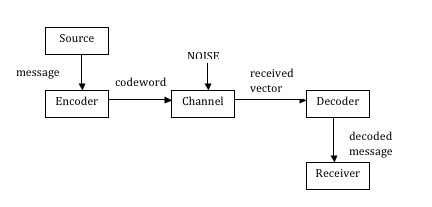
\includegraphics[scale=1.00]{PNGs/figure1_1_comm_link}
\end{figure}


\begin{example}
Suppose we are using an alphabet containing only two symbols, say 0 and 1 and we wish to
send a message to a friend of either ``YES'' or ``NO''.  We first might consider encoding 1 for ``YES'' and
0 for ``NO''; however, if the codeword 0 is sent and then altered by the channel to be received as 1, the
decoder will incorrectly pass the message �YES� to the receiver.  One way of improving the situation is to
add redundancy by repeating the symbol.  For instance, we might encode ``YES'' as the codeword 11 and ``NO''
as 00.  Now if �NO� is sent, two errors would have to occur before the decoder returns an incorrect message.
If one error occurs then the received vector will either be 10 or 01, neither of which is a codeword.  At
this point, the receiver might request a retransmission.  This is an example of a code in which one error
may be detected.  To strengthen the code to be error-correcting we might increase the redundancy by repeating
the message five times.  Thus we encode our message ``NO'' as 00000.  Perhaps the channels interferes to cause
the decoder to receive the vector 00110.  Using the method of nearest neighbor decoding the decoder assesses
the message and decides that of the two possible codewords (i.e. 00000 and 11111) 00000 is more likely the
one originally sent and hence is correctly decoded as ``NO''.
\end{example}

\begin{assumption}
Implicit in our example are two assumptions.  First, we are assuming that each symbol is equally likely to
occur.  Second, the probability of an error is less than $1/2$.  These are important assumptions to
be aware as they will serve as guiding principles in the remainder of this paper.
\end{assumption}
      
\begin{definition}
Let $\mathbf{F}$ be a finite set, or {\bf alphabet}, of $q$ elements.  A
$q$-{\bf ary code} $\mathbf{C}$ is a set of finite sequences of symbols of $\mathbf{F}$, called {\bf codewords}
and written $x_1x_2\cdots x_n$, or $(x_1,x_2,\ldots,x_n)$, where $x_i\in \mathbf{F}$ for $i = 1,\ldots,n$.
If all the sequences have the same length $n$, then $\mathbf{C}$ is a {\bf block code} of {\bf block length}
$n$.\\
\end{definition}


Given an alphabet $\mathbf{F}$, it is consistent with terminology for vector spaces when $\mathbf{F}$ is a
field to denote the set of all sequences of length $n$ of elements of $\mathbf{F}$ by $\mathbf{F}^n$
and to call these sequences vectors.  The member of $\mathbf{F}$ at the $i$th position of a vector is
known as the coordinate at $i$.\\

\begin{definition}
Let $v=(v_1,v_2,\ldots,v_n)$ and $w=(w_1,w_2,\ldots,w_n)$ be two vectors in $\mathbf{F}^n$. 
The {\bf Hamming distance}, $d(v,w)$, between $v$ and $w$ is the number of coordinate places in which they differ:

$$
d(v,w)=\{i|v_i\neq w_i \}
$$


We will usually refer to the Hamming distance as simply the {\bf distance} between two vectors.\\
\end{definition}

{\bf Nearest-neighbor decoding} is a method in which the received vector is translated as the codeword of
smallest distance, whenever it is uniquely determined.  This method maximizes the likelihood of correcting
errors provide the two assumptions mentioned above hold (i.e. probability of an error $<1/2$ and each
symbol is equally likely to be transmitted).

\begin{definition}
The {\bf minimum distance} $d(\mathbf{C})$ of a code $\mathbf{C}$ is the smallest of the
distances between distinct codewords; i.e.

$$
d(\mathbf{C}) = \min\{d(v,w)|v,w\in\mathbf{C},v\neq w\}
$$
\end{definition}


\begin{example}
The error-correcting code in this example is a binary code of block length 5.
The distance between the codeword 00000 and the received vector 00110 is 2.  The distance between the same
received vector and the codeword 11111 is 3.  Thus, 00000 is the nearest neighboring codeword.  The minimum
distance of this code is 5.
\end{example}

\begin{definition}
A code $\mathbf{C}$ over $\mathbf{F}$ of length $n$ is {\bf linear} if $\mathbf{C}$ is a
subspace of the vector space $V=\mathbf{F}^n$.  If $\dim(\mathbf{C})=k$ and $d(\mathbf{C})=d$, then we write
$[n,k,d]$ for the $q$-ary code $\mathbf{C}$; if the minimum distance is not specified we simply write $[n,k]$.
The {\bf information rate} is $k/n$ and the {\bf redundancy} is $n-k$.  
\end{definition}

Since $\mathbf{C}$ is a subspace, it follows that the {\bf all-zero} vector must be a codeword in $\mathbf{C}$
also the sum of any two codewords must also be a codeword in $\mathbf{C}$.  We will also see after the next
definition that the distance $d$ is also easy to calculate for linear codes.\\

\begin{definition}
Let $V=F^n$.  For any vector $v=(v_1,v_2,\ldots,v_n)$  $V$ set

$$
S=\left\{i|v_i\neq 0\right\}
$$
\end{definition}


Then $S$ is called the support of $v$ and the weight of $v$ is $\left|S\right|$.  The {\bf minimum weight}
of a code is the minimum of the weights of the nonzero codewords.\\

\begin{theorem}
Let $\mathbf{C}$ be a $[n,k,d]$ code.  Then the minimum distance $d = d(\mathbf{C})$,
is the minimum weight of $\mathbf{C}$.\\
\end{theorem}


\begin{pf}
Notice that in $F^n$, $d(v,w)=\mathbf{wt}(v - w)$.  Since $\mathbf{C}$ is a subspace $v-w\in \mathbf{C}$
for any $v,w\in\mathbf{C}$.\\
\end{pf}

\begin{example}\label{hamming}
Listed below are all 16 codewords in the linear $[7,4,3]$ binary code.  They are listed in order
of increasing weight.\\

\begin{center}
 \begin{tabular}{cccc}
  0000000 & 0111000 & 1000111 & 0101101\\
  1100100 & 0001110 & 1101010 & 0110110\\
  1010010 & 0010101 & 1110001 & 0011011\\
  1001001 & 0100011 & 1011100 & 1111111\\
 \end{tabular}
\end{center}

Notice that the minimum weight is 3.  By Theorem 1.1 it follows that $d(\mathbf{C}) = 3$.  It can be shown
that these 16 codewords form a subspace of $\mathbf{F}^7$ with basis $\{(1,0,0,0,1,1,1)$, $(0,1,0,0,0,1,1)$,
$(0,0,1,0,1,0,1)$, $(0,0,0,1,1,1,0)\}$. Thus $\dim(\mathbf{C})=4$ as conveyed in the notation and the
redundancy is 3 since $n-k=7-4 = 3$.
\end{example}

If we look closer at Example \ref{hamming}, we find that there are 7 vectors of weight 3.  Isolating our attention to
only these 7 vectors, we notice that these make up the rows of the 7 x 7 incidence matrix of the Fano Plane
(see Figure \ref{fano_plane}).  The 7 vectors of weight 4 are the compliments of the weight 3 vectors.  That is, these
vectors make up the rows of the 7 x 7 matrix that indicates which 4 points are not on each line (i.e. $l_1$,
$l_2$, $l_3$, $l_4$ $l_5$, $l_6$, $l_7$)\\

\begin{theorem}
Let $\mathbf{C}$ be a code of minimum distance $d$.  If $d=2t+1$, then $\mathbf{C}$ can
be used to correct up to $t$ errors.\\
\end{theorem}


\begin{corollary}
If $d(\mathbf{C})=d$ then $\mathbf{C}$ can be used to correct up to $[(d - 1)/2]$ errors.\\
\end{corollary}

\begin{figure}[h!]
\caption{The Fano Plane}
\label{fano_plane}
\centering
  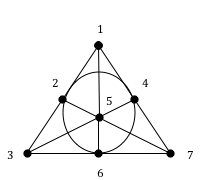
\includegraphics[scale=1.00]{PNGs/Fano_Plane_of_order_2}
\end{figure}


\begin{center}
Incidence Matrix

\begin{tabular}{c|ccccccc}
  & l1 & l2 & l3 & l4 & l5 & l6 & l7\\
\hline
1 & 1  & 1  & 0  & 0  & 1  & 0  & 0\\
2 & 1  & 0  & 1  & 0  & 0  & 1  & 0\\
3 & 1  & 0  & 0  & 1  & 0  & 0  & 1\\
4 & 0  & 1  & 1  & 1  & 0  & 0  & 0\\
5 & 0  & 0  & 0  & 1  & 1  & 1  & 0\\
6 & 0  & 0  & 1  & 0  & 1  & 0  & 1\\
7 & 0  & 1  & 0  & 0  & 0  & 1  & 1\\
\end{tabular}
\end{center}

\vspace{15pt}

\begin{definition}
A code $\mathbf{C}$ is said to be a perfect t-error correcting code if any vector $v$ in
$\mathbf{F}^n$ can be corrected to a exactly one codeword in $\mathbf{C}$ should the distance between $v$ and
the codeword be less than or equal to $t$.\\
\end{definition}

\begin{example}
Since $d(\mathbf{C})=3$, this $[7,4,3]$ binary code may be used to correct 1
error, should it occur. This code is a perfect single-error-correcting code known as a Hamming code.  Hamming
codes have the nice property of being very easy to decode.  A method which we will not explore here.  It turns
out that the inner product of any one of the weight-3 vectors of this code with any one of the weight-4 vectors
results in the all-zero vector.  This means that the 7 weight-4 vectors of this code are in the nullspace of
$\mathbf{C}$.  In fact, the 3 vectors $(1,1,0,1,0,1,0)$, $(1,1,0,0,0,0,1)$, and $(1,0,1,1,1,0,0)$ make up a
basis
\end{example}



\begin{figure}[h!]
\caption{Biplane of order 2}
\label{biplane}
\centering
  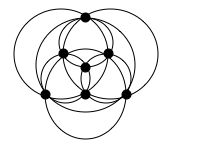
\includegraphics[scale=1.00]{PNGs/Biplane_of_order_2}
\end{figure}

\begin{center}
Incidence Matrix

\begin{tabular}{c|ccccccc}
  & l1 & l2 & l3 & l4 & l5 & l6 & l7\\
\hline
1 & 1  & 0  & 0  & 0  & 1  & 1  & 1\\
2 & 1  & 1  & 0  & 1  & 0  & 1  & 0\\
3 & 0  & 1  & 0  & 1  & 1  & 0  & 1\\
4 & 1  & 0  & 1  & 1  & 1  & 0  & 0\\
5 & 1  & 1  & 1  & 0  & 0  & 0  & 1\\
6 & 0  & 1  & 1  & 0  & 1  & 1  & 0\\
7 & 0  & 0  & 1  & 1  & 0  & 1  & 1\\
\end{tabular}
\end{center}

\vspace{15pt}

Figure \ref{biplane} for the nullspace of $\mathbf{C}$.  These three vectors may be used to make up the rows of
what is known as a Parity Check Matrix $H$ for this Hamming code.  This matrix $H$ plays an important role in
the decoding of this binary code (Hill, 1991).\\

Figure \ref{biplane} shows the geometry for the biplane of order 2 (Polster, 1998) and its associated incidence
matrix.  This geometry is the compliment to the Fano plane.  Each circle represents a line in the geometry
containing four points. Notice the 7 rows of the incidence for this geometry are precisely the 7 weight-4
vectors of our Hamming code (Assmus and Key,1992).\\


\begin{proposition}
The minimum-weight vectors of any linear perfect code generate the code.\\
\end{proposition}

\begin{example}
By this proposition we see that the Fano Plane generates this Hamming code.  As we
mentioned above the biplane of order 2 generates the nullspace to this code and not the
entire code itself.
\end{example}

\begin{ques}
What happens when take the 13 row vectors of the incidence matrix for the Projective Plane of
order 3?  Since the dimension of this matrix is 12, do we get a perfect [13,12,4] single error-correcting code?
If not, what code is obtained by using this incidence structure?
\end{ques}


\section{Conclusion}
An example of a code has been given which is entirely generated by the projective plane of order 2.
We have seen the power of linear codes, a result that stems from the fact that they are vector subspaces.  Every
subspace of a finite-dimensional vector space has an associated projective (finite) geometry. So it seems only
natural that finite geometries might be an ideal source in establishing error-correcting linear codes.


%References
%	Assmus, E.F. and Key, J.D. (1992), DESIGNS AND THEIR CODES, Cambridge University Press, New York, NY
%	Hill, R. (1991), A FIRST COURSE IN CODING THEORY, Oxford University Press, NY
%      Polster, B. (1998), A GEOMETRICAL PICTURE BOOK, Springer-Verlag, New York, NY
\end{document}
